\chapter{등가 원리에서 텐서까지}

일반상대성이론은 흔히 GR로 줄여 부르지만, 특수상대성이론을 SR이라고 부르는 경우는 드물다. 약칭보다 중요한 것은 처음부터 시작하기로 하는 선택이다. 가장 직접적인 길은 아인슈타인이 택한 길이다. 엘리베이터 안에서 체감할 수 있을 만큼 단순한 물리적 관찰에서 출발해 그 결과가 불가피해질 때까지 밀고 나간 다음, 비로소 기하학을 도입한다.

첫 번째 관찰은 등가 원리다. 중력과 가속은 국소적으로 구별할 수 없다. 여기서 ‘국소적’이라는 말은 결국 이 명제의 거의 모든 내용을 떠맡게 된다. 그러나 그 말의 의미를 한정하기에 앞서, 한정하지 않은 명제만으로 무엇을 할 수 있는지 살펴보자.

\section{좌표 변환으로서의 엘리베이터}

교과서에서는 아인슈타인의 엘리베이터를 흔히 로켓으로 바꾸어 설명한다. 여기서는 가속이 익숙한 엘리베이터가 더 적절하다. 지면에 붙어 있는 기준계에서 높이를 \(z\)로, 엘리베이터 바닥에서 잰 높이를 \(z'\)로 나타내자. 바닥의 높이가 \(L(t)\)라면, 같은 사건의 좌표는 다음과 같다.
\begin{equation}
 z'=z-L(t),\qquad t'=t,\qquad x'=x.
\label{eq:elevator-map}
\end{equation}
엘리베이터가 옆으로 미끄러지지 않으므로 수평 좌표는 변하지 않는다. 당분간 특수상대성이론을 의도적으로 배제하기 위해 \(t'=t\)로 둔다.

\begin{classroomqa}
\audiencequestion{특수상대성이론을 무시하면서 일반상대성이론 강의를 어떻게 시작할 수 있습니까?}
\lecturerresponse{중요한 중력 효과가 나타나면서도 모든 속도가 \(c\)보다 훨씬 작은 영역이 있다. 따라서 중력과 가속의 연관성--을 뉴턴 역학에서 따로 살펴본 뒤 민코프스키 기하학과 결합할 수 있다. 이는 설명을 위한 단계적 선택이지, 최종 이론이 비상대론적이라는 주장이 아니다. \lecturetimestamp{00:05:33}}
\end{classroomqa}

두 관성계 사이에서 엘리베이터가 등속 운동한다고 하자.
\begin{equation}
 L(t)=vt,\qquad z'=z-vt.
\label{eq:galilean-elevator}
\end{equation}
두 좌표계의 원점은 \(t=0\)에 일치하도록 정했다. 판서에는 엘리베이터 그림을 세 가지 좌표 관계와 나란히 두어 기호가 물리적 의미를 잃지 않도록 한다.

\begin{figure}[H]
\centering
\includegraphics[width=\linewidth]{lecture_01_figure_01.png}
\caption{등속도 특수화 후의 엘리베이터 좌표 \(L(t)=vt\).}
\par\smallskip
\textit{강의 프레임: 00:09:10.}
\end{figure}

뉴턴 법칙의 수직 성분만 생각하자.
\begin{equation}
 F=m\ddot z.
\label{eq:newton-unprimed}
\end{equation}
힘은 밧줄, 전기장 또는 다른 통상적인 상호작용에서 비롯될 수 있다. \eqref{eq:galilean-elevator}을 두 번 미분하면
\(\ddot z'=\ddot z\)가 되고, 따라서
\begin{equation}
 F=m\ddot z'.
\label{eq:newton-primed-inertial}
\end{equation}
법칙의 형태는 변하지 않는다. 이 간단한 계산은 관성계 등가성의 실제 내용을 드러낸다. 선형 좌표 변환은 등속 운동을 등속 운동으로 보낸다.

\begin{figure}[H]
\centering
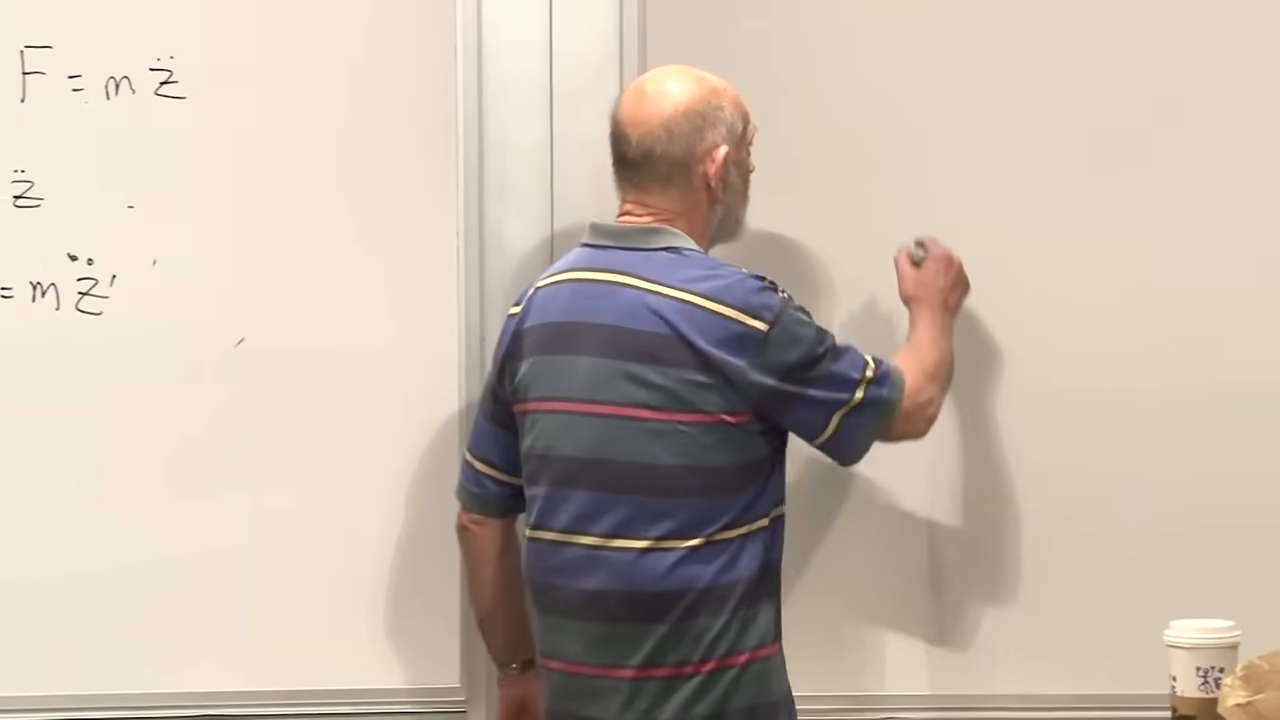
\includegraphics[width=\linewidth]{lecture_01_figure_02.png}
\caption{등속 운동하는 두 좌표계에서의 뉴턴 방정식.}
\par\smallskip
\textit{강의 프레임: 00:11:50.}
\end{figure}

이제 엘리베이터가 일정한 \(g\)로 위쪽을 향해 가속한다고 하자.
\begin{equation}
 L(t)=\frac12gt^2,\qquad
 \dot L=gt,\qquad
 \ddot L=g.
\end{equation}
좌표 변환은 다음과 같이 된다.
\begin{equation}
 z'=z-\frac12gt^2,
\qquad
 \ddot z'=\ddot z-g.
\label{eq:accelerated-map}
\end{equation}
이를 뉴턴 법칙에 대입하면
\begin{equation}
 F=m(\ddot z'+g),
\qquad
 m\ddot z'=F-mg.
\label{eq:fictitious-gravity}
\end{equation}
유도 과정에는 유용한 부호 점검이 포함되어 있다. \(+mg\)는 처음에 가속도 쪽에 나타나며, 힘 쪽으로 옮길 때에만 \(-mg\)가 된다. 엘리베이터 바닥이 위쪽으로 가속하는 기준계에서 최종 힘의 방향은 아래쪽이다.

\begin{figure}[H]
\centering
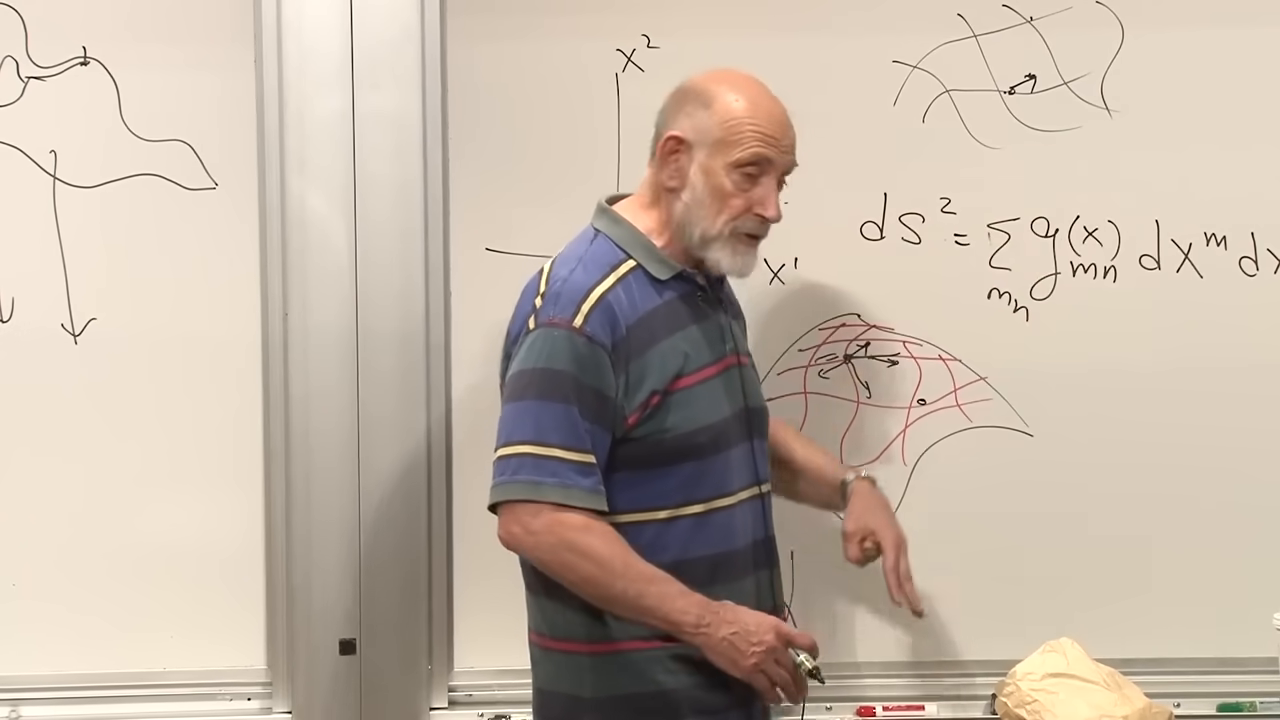
\includegraphics[width=\linewidth]{lecture_01_figure_03.png}
\caption{가속 좌표 변환과 그에 따른 가상 힘 \(-mg\).}
\par\smallskip
\textit{강의 프레임: 00:15:35.}
\end{figure}

새 항이 중력처럼 보이는 데에는 정확한 이유가 있다. 질량에 비례하기 때문이다. 관성에 대한 반응 역시 질량에 비례하므로 운동 방정식에서 질량은 소거된다. 자유낙하하는 물체는 질량과 무관하게 같은 궤적을 따른다. 예를 들어 시험체 근사에서는 지구의 궤도가 지구 자체의 질량이 아니라 태양의 중력장 안에서의 위치와 속도로 정해진다.

아인슈타인 이전에는 이 유사성을 단순한 흥미거리로 치부할 수 있었다. 그러나 아인슈타인은 이를 원리로 격상했다. 국소적인 기계 실험으로는 균일한 중력장과 적절히 가속하는 기준계를 구별할 수 없다.

\section{직선, 곡선 좌표와 빛}

세로축에 \(t\)를, 가로축에 \(z\)를 놓자. \(z'=z-vt\)일 때 \(z'\)가 일정한 선은 서로 평행한 직선이다. 좌표 변환이 선형이므로 직선 세계선은 변환 후에도 직선이다.

\begin{figure}[H]
\centering
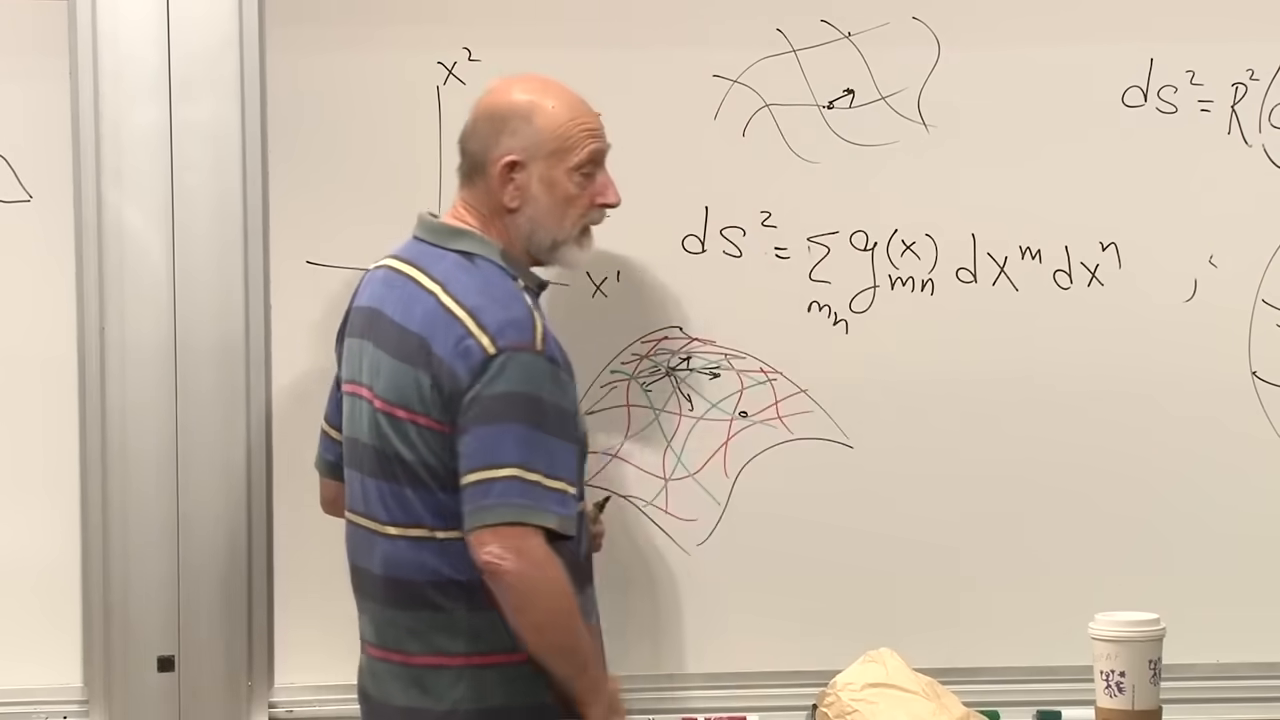
\includegraphics[width=\linewidth]{lecture_01_figure_04.png}
\caption{등속 운동 좌표계에 대한 선형 시공간 격자.}
\par\smallskip
\textit{강의 프레임: 00:19:45.}
\end{figure}

가속 좌표 변환에서는 \(z'\)가 일정한 선이 다음 관계를 만족한다.
\begin{equation}
 z=z'+\frac12gt^2.
\end{equation}
옆으로 누운 포물선이다. 운동을 과거 방향으로 연장하면 엘리베이터는 하강하면서 감속하고, 방향을 바꾼 뒤 위쪽으로 가속한다. 서로 이웃한 \(z'\) 일정선은 모두 같은 포물선을 가로 방향으로 평행 이동한 것이다.

\begin{figure}[H]
\centering
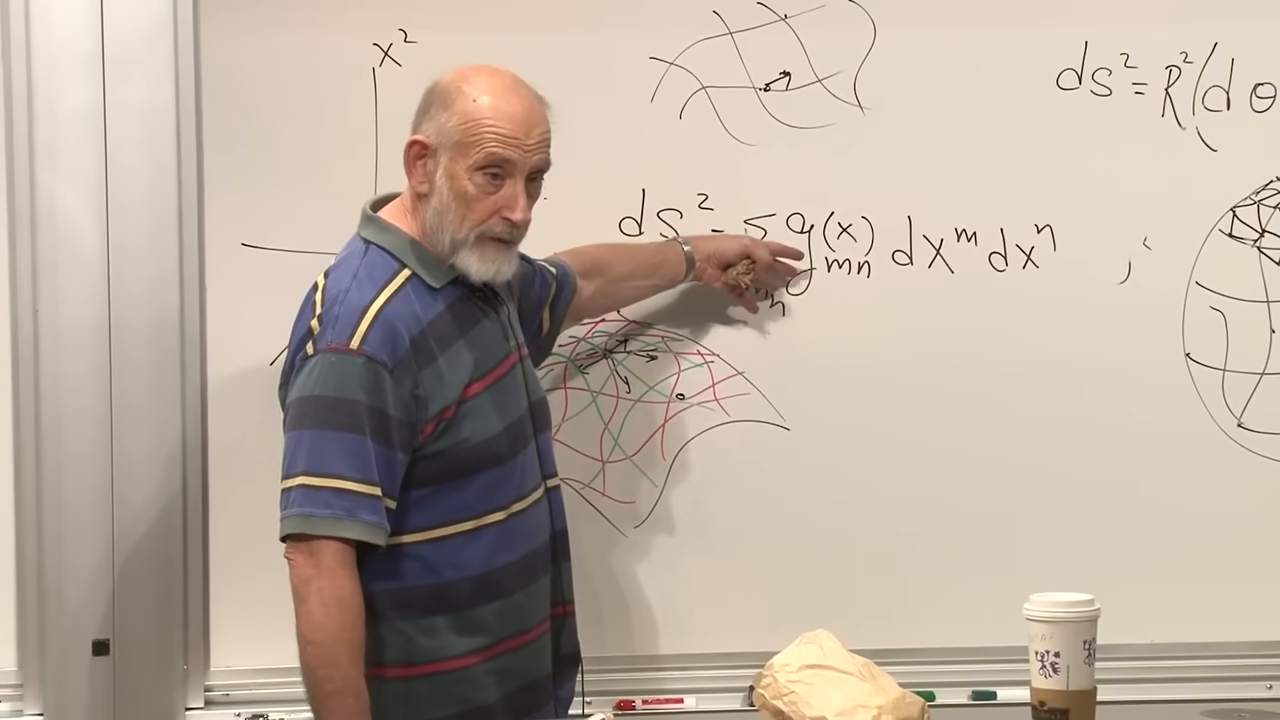
\includegraphics[width=\linewidth]{lecture_01_figure_05.png}
\caption{등가속 좌표계에서 \(z'\)가 일정한 곡선들.}
\par\smallskip
\textit{강의 프레임: 00:22:25.}
\end{figure}

여기서 첫 번째 기하학적 단서를 얻는다. 특수상대성이론의 선형 로런츠 변환은 시공간의 직선을 다른 직선으로 보낸다. 가속을 나타내어 중력을 모사하려면 시공간 좌표의 곡선형 변환이 필요하다.

아인슈타인은 이처럼 사소해 보이는 점을 이용해 결코 사소하지 않은 질문에 답했다. 중력은 빛에 영향을 미치는가? \(t=0\) 엘리베이터와 지면 기준계가 순간적으로 서로 정지해 있다고 하고, 엘리베이터를 가로질러 수평으로 빛을 보낸다. 가속하지 않는 기준계에서는
\begin{equation}
 x=ct,\qquad z=0.
\end{equation}
\(z=z'+\tfrac12gt^2\)를 이용하면 같은 빛이 엘리베이터 좌표에서 다음 관계를 따른다.
\begin{equation}
 z'=-\frac12gt^2
    =-\frac{g}{2c^2}x^2.
\label{eq:accelerated-light}
\end{equation}
관성계에서는 빛의 궤적이 직선이고 가속계에서는 곡선이다. 가속과 중력이 국소적으로 등가라면 중력장은 빛을 휘게 해야 한다. 이 논증은 중력의 장 방정식을 쓰기도 전에 그 효과를 확립한다.

\begin{figure}[H]
\centering
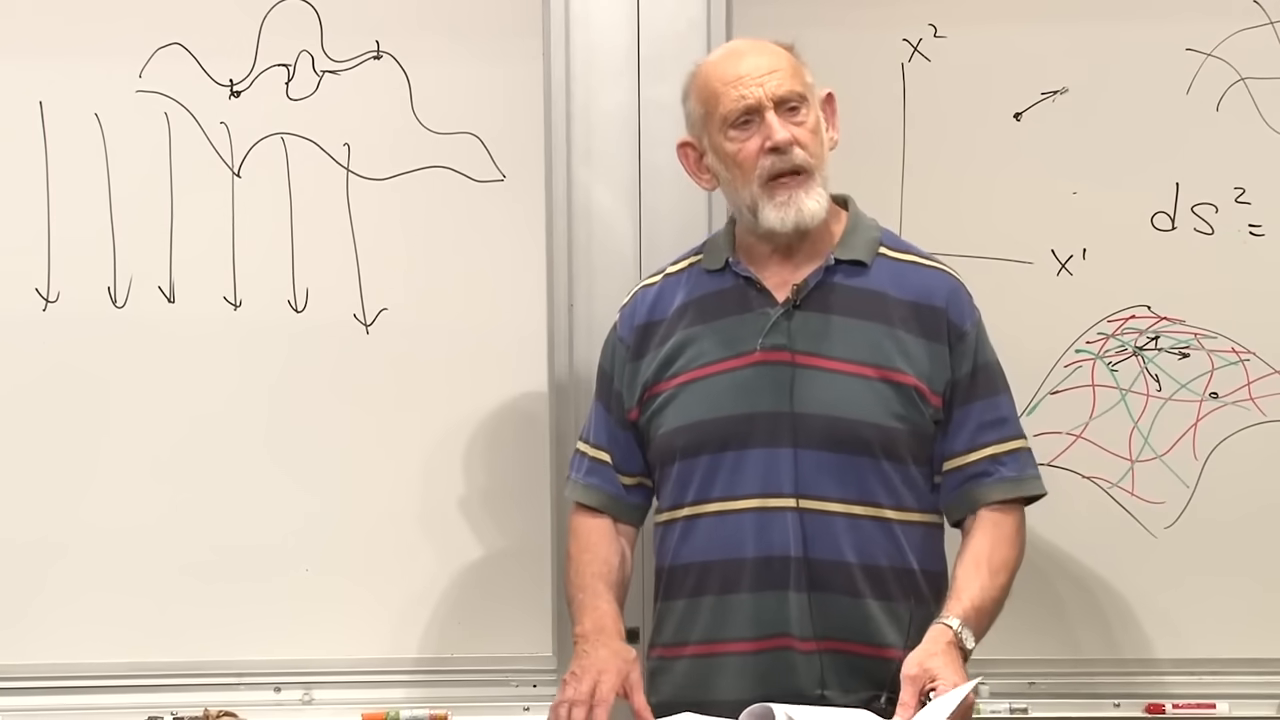
\includegraphics[width=\linewidth]{lecture_01_figure_06.png}
\caption{수평 광선과 가속 기준계에서의 곡선 궤적.}
\par\smallskip
\textit{강의 프레임: 00:28:10.}
\end{figure}

\section{좌표 변환으로 없앨 수 없는 것}

가속 기준계는 겉보기의 균일한 중력장을 만들어 낼 수 있다. 그렇다고 모든 중력장이 좌표 선택의 산물이라는 뜻은 아니다. 별의 중력장은 반지름 방향 안쪽을 향한다. 별 가까이의 한 지점에서 작은 자유낙하 실험실의 국소 가속을 없앨 수는 있지만, 같은 변환으로 별의 모든 방향에 걸친 장을 없앨 수는 없다.

\begin{figure}[H]
\centering
\includegraphics[width=\linewidth]{lecture_01_figure_07.png}
\caption{조석 가속을 드러내기 위한 반지름 방향 장과 길게 뻗은 낙하 물체.}
\par\smallskip
\textit{강의 프레임: 00:32:50.}
\end{figure}

이를 가로막는 것은 조석력이다. 길이가 2천 마일인 사람이 발부터 먼저 떨어진다고 상상해 보자. 발이 중력원에 더 가까워 머리보다 더 큰 가속을 받으므로 몸이 늘어난다. 옆으로 눕히면 양쪽에서 안쪽을 향하는 방향의 성분이 서로를 향하므로 몸이 압축된다. 뉴턴 역학으로 말하면, \(\xi^j\)만큼 떨어진 이웃한 점들은 상대 가속도
\begin{equation}
 \delta a^i \simeq \partial_j g^i\,\xi^j.
\label{eq:newtonian-tide}
\end{equation}를 얻는다.
좌표에 따른 가속도는 없앨 수 있다. 그러나 유한한 크기를 가진 자유낙하 물체 안에서 나타나는 상대 가속은 없앨 수 없다.

\begin{classroomqa}
\audiencequestion{머리와 발에 서로 다른 로켓 엔진을 달아 늘어나는 효과를 흉내 내고, 따라서 조석장도 모사할 수 있습니까?}
\lecturerresponse{엔진을 작동하면 물체에 실제로 응력이 가해질 수는 있지만, 그것은 물체의 각 부분에 다르게 작용하는 비중력 힘이다. 좌표 변환만으로는 이웃한 자유낙하 입자들 사이의 불변 상대 가속을 만들어 낼 수 없다. 이 판별 기준은 자유낙하 상태에 힘을 가하지 않은 경우에 관한 것이지, 각기 다른 로켓으로 추진하는 물체에 관한 것이 아니다.
\lecturetimestamp{00:36:51}}
\end{classroomqa}

곡선 좌표를 쓰면 가상장이 훨씬 복잡해 보일 수 있다. 기준계가 수직으로 가속하는 동시에 수평으로 진동하면 두 성분을 모두 가진 시간 의존적 겉보기 장이 생긴다. 일상적인 극좌표도 유익한 예다. 직선인 카르테시안 궤적을 따라 움직이는 자유 입자는 먼저 \(r(t)\)가 감소하고, 최소 반지름에 이른 다음 \(r(t)\)가 증가한다. \(r(t)\)와 \(\theta(t)\)만 본 사람은 바깥쪽으로 밀어내는 반발력이 있다고 추론할 수도 있다. 이 좌표를 회전시키면 원심력 항과 코리올리 항도 나타난다. 이 항들은 질량에 비례해 중력처럼 보이지만, 자유낙하 물체에 불변인 조석 변형을 남기지는 않는다.

\begin{classroomqa}
\audiencequestion{운동을 각좌표나 극좌표로 나타내면 어떻게 됩니까?}
\lecturerresponse{비선형 좌표 표현에서는 직선 자유 궤적이 마치 입자가 \(r=0\)에서 밀려나는 것처럼 보인다. 이 유효 원심력은 좌표에 따른 힘이다. 관성 카르테시안 기준계로 돌아가면 이 힘은 사라지고 조석 변형이 없다는 사실이 드러난다.
\lecturetimestamp{00:37:56}}
\end{classroomqa}

\begin{figure}[H]
\centering
\includegraphics[width=\linewidth]{lecture_01_figure_08.png}
\caption{직선 궤적의 극좌표 표현. 판서에는 \(r(t)\)와 \(\theta(t)\)가 표시되어 있다.}
\par\smallskip
\textit{강의 프레임: 00:40:20.}
\end{figure}

\begin{classroomqa}
\audiencequestion{여러 중력원의 효과가 서로 상쇄되어 조석력이 사라질 수 있습니까?}
\lecturerresponse{특정 지점에서는 힘이 상쇄될 수 있지만, 장의 값이 상쇄된다고 해서 공간 미분까지 일반적으로 상쇄되는 것은 아닙니다. 각 원천 가까이에서는 이웃한 궤적들이 여전히 서로 다른 가속도를 얻습니다. 곡률이 실제로 없으려면 특정 지점의 알짜힘이 0인 것만으로는 부족하며, 그 영역 전체에서 조석 진단량이 사라져야 합니다. \lecturetimestamp{00:42:16}}
\end{classroomqa}

\begin{classroomqa}
\audiencequestion{조석력은 실제로 어떻게 측정합니까?}
\lecturerresponse{결정 같은 유한한 크기의 물체를 자유낙하시켜 한 방향으로 늘어나고 다른 방향으로 압축되는 응력과 변형이 생기는지 살펴본다. 이런 변형은 측정할 수 있으며 좌표 이름을 바꿔도 사라지지 않는다. \lecturetimestamp{00:44:38}}
\end{classroomqa}

\begin{classroomqa}
\audiencequestion{회전목마에 탄 2천 마일 길이의 사람은 반지름 방향 조석 효과를 느끼게 됩니까?}
\lecturerresponse{회전목마에 묶인 사람은 지지력을 느끼며 실제로 두통이 생길 수도 있다. 그러나 시험 물체는 자유낙하 상태여야 한다. 회전 좌표에서는 궤적이 복잡해 보이지만, 관성계에서는 응력을 받지 않는 직선 궤적을 따르므로 불변 조석력은 0이다.
\lecturetimestamp{00:45:07}}
\end{classroomqa}

\begin{classroomqa}
\audiencequestion{낙하하는 물체의 방향을 기울이면 늘어나는 효과와 압축되는 효과가 상쇄됩니까?}
\lecturerresponse{물체의 전체 변형을 없애는 단일한 방향은 없다. 반지름 방향 장은 한 주축 방향으로 물체를 늘리고 횡방향으로 압축한다. 모든 방향으로 유한한 크기를 가진 물체는 이 전체 변형 양상을 겪는다. \lecturetimestamp{00:47:10}}
\end{classroomqa}

\begin{figure}[H]
\centering
\includegraphics[width=\linewidth]{lecture_01_figure_09.png}
\caption{유한한 크기의 자유낙하 물체에서 반지름 방향 신장과 횡방향 압축을 함께 나타낸 그림.}
\par\smallskip
\textit{강의 프레임: 00:47:55.}
\end{figure}

\begin{classroomqa}
\audiencequestion{조석력이 있다는 것은 등가 원리가 성립하지 않는다는 뜻입니까?}
\lecturerresponse{조석력은 등가 원리를 얼마나 주의 깊게 진술해야 하는지를 알려 준다. 중력장이 계의 범위 안에서 무시할 수 있을 만큼만 변하는 작은 계에서는 자유낙하 기준계를 사용해 필요한 정확도까지 중력을 없앨 수 있다. 더 큰 계의 범위에 걸친 잔여 변화가 조석장이다. \lecturetimestamp{00:48:08}}
\end{classroomqa}

\section{민코프스키 기하학에서 국소 계량으로}

이제 잠시 중력에서 벗어나자. 민코프스키는 시공간에 불변인 국소 기하학이 있음을 이미 보여 주었다. \(c=1\)인 한 공간 차원에서는
\begin{equation}
 d\tau^2=dt^2-dx^2.
\label{eq:minkowski-proper-time}
\end{equation}
대신 \(ds^2=dx^2-dt^2=-d\tau^2\)로 정의할 수도 있다. 두 표현의 차이는 부호수 관례에 있을 뿐 물리학의 차이가 아니다.

\begin{classroomqa}
\audiencequestion{빛의 속도를 1로 두지 않는다면 그 값은 어디에 들어갑니까?}
\lecturerresponse{시간 단위로 \(t\)를, 길이 단위로 \(x\)를 측정한다면 편리한 표현 하나는 다음과 같다.
\(d\tau^2=dt^2-dx^2/c^2\). 여기에 \(c^2\)를 곱해 다음과 같이 쓸 수도 있다.
\(c^2d\tau^2=c^2dt^2-dx^2\). \(ct\) 또는 \(x/c\)를 좌표로 택하면 환산 인자가 흡수된다. \lecturetimestamp{00:51:02}}
\end{classroomqa}

\begin{figure}[H]
\centering
\includegraphics[width=\linewidth]{lecture_01_figure_10.png}
\caption{특수상대성이론에서 일반상대성이론으로 이어지는 기하학적 연결을 제공하는 고유시간 간격.}
\par\smallskip
\textit{강의 프레임: 00:51:10.}
\end{figure}

아인슈타인은 중력장을 없앨 수 있는지 판별하는 문제가 가우스가 곡면에 대해, 리만이 임의 차원에 대해 연구한 문제와 닮았음을 알아차렸다. 국소적인 거리 법칙이 주어졌을 때, 기하학이 실제로 휘어 있는지를 어떻게 판별할 수 있을까?

유클리드 카르테시안 좌표에서는 피타고라스 정리에 따라
\begin{equation}
 ds^2=(dx^1)^2+(dx^2)^2+\cdots
     =\delta_{mn}\,dx^m dx^n.
\label{eq:euclidean-line-element}
\end{equation}
지표의 범위가 공간의 차원이다. 좌표가 2개든 3개든 26개든 표기법은 달라지지 않는다.

\begin{figure}[H]
\centering
\includegraphics[width=\linewidth]{lecture_01_figure_11.png}
\caption{좌표 미소 변화의 제곱을 더한 유클리드 선요소.}
\par\smallskip
\textit{강의 프레임: 00:55:00.}
\end{figure}

임의의 곡면 위에 임의의 좌표 \(x^m\)를 놓자. 서로 이웃한 두 점 사이의 거리는 다음 이차 형식으로 주어진다.
\begin{equation}
 ds^2=g_{mn}(x)\,dx^m dx^n.
\label{eq:general-line-element}
\end{equation}
함수 \(g_{mn}(x)\)는 계량 텐서의 성분이다. 이 같은 식은 곡선 좌표로 나타낸 평평한 곡면에도 적용된다. 계량 성분이 일정하지 않다는 사실만으로는 내재 곡률이 있음을 증명할 수 없다.

\begin{figure}[H]
\centering
\includegraphics[width=\linewidth]{lecture_01_figure_12.png}
\caption{곡선 좌표망과 나란히 나타낸 일반적인 계량 이차 형식.}
\par\smallskip
\textit{강의 프레임: 00:58:20.}
\end{figure}

반지름이 \(R\)인 구에서 \(\theta\)를 극으로부터 잰 각이라 하면
\begin{equation}
 ds^2=R^2\left(d\theta^2+\sin^2\theta\,d\phi^2\right).
\label{eq:sphere-polar}
\end{equation}
같은 경도 변화도 적도 부근에서는 긴 거리에, 극 부근에서는 짧은 거리에 해당한다. 계수는 바로 이 위치 의존성을 나타낸다.

\begin{classroomqa}
\audiencequestion{일반적인 위도는 적도에서부터 재는데, 그러면 계수는 사인 대신 코사인이 되어야 하지 않습니까?}
\lecturerresponse{그렇다. \(\lambda\)가 적도에서부터 잰 위도라면
\(ds^2=R^2(d\lambda^2+\cos^2\lambda\,d\phi^2)\)이다.
\eqref{eq:sphere-polar}에서는 북극에서부터 잰 극각 \(\theta=\pi/2-\lambda\)를 사용한다.
\lecturetimestamp{01:01:03}}
\end{classroomqa}

\begin{figure}[H]
\centering
\includegraphics[width=\linewidth]{lecture_01_figure_13.png}
\caption{구의 계량과 위치에 따른 계수를 정해 주는 위도--경도 기하학.}
\par\smallskip
\textit{강의 프레임: 01:00:30.}
\end{figure}

더 일반적인 좌표에서는 \(d\theta\,d\phi\) 교차항이 생길 수 있지만, 국소 거리는 여전히 미분량에 대한 이차식이다. 리만 계량의 선요소에는 삼차항이나 일차항이 들어가지 않는다.

\section{국소 거리와 내재 곡률}

\begin{classroomqa}
\audiencequestion{계량 공식은 서로 멀리 떨어진 두 점 사이의 거리도 주나요?}
\lecturerresponse{그대로 대입해서 구할 수는 없다. 이 공식은 서로 이웃한 점 사이의 거리를 준다. 거시적인 거리를 구하려면 경로를 정하고 \(ds\)를 적분해야 한다. 거리가 최단 경로를 뜻한다면 그 경로 자체도 기하학으로부터 찾아야 한다. 같은 두 끝점을 잇는 국소 최단 경로가 여럿일 수도 있다. \lecturetimestamp{01:02:30}}
\end{classroomqa}

울퉁불퉁한 곡면 위 서로 멀리 떨어진 두 점에 말뚝을 박고 그 사이에 팽팽한 줄을 놓는다고 상상해 보자. 줄은 언덕의 한쪽이나 다른 쪽을 돌아갈 수 있으며, 언덕을 옮기면 길이를 최소화하는 경로도 달라진다. 전체 거리는 그 사이 공간의 기하학에 달려 있다. 국소 거리는 더 간단하다. 계량은 각 점에 작은 자를 제공하고, 기하학은 이 무한소 자들을 모아 구성된다.

\begin{figure}[H]
\centering
\includegraphics[width=\linewidth]{lecture_01_figure_14.png}
\caption{전체 거리의 문제: 팽팽한 경로는 양 끝점 사이의 곡면을 따라가야 한다.}
\par\smallskip
\textit{강의 프레임: 01:04:00.}
\end{figure}

국소적인 조각들을 늘이거나 찢지 않고 평면 위에 펼칠 수 있다면 내재 기하학은 평평하다. 삼각분할한 구의 변 길이를 가진 조각들은 모서리를 보존하면서 모두 평평하게 펼칠 수 없다. 따라서 계량은 다음과 같은 명확한 문제를 제기한다. \(g_{mn}(x)\)가 주어졌을 때, 무한소 조각들이 평평한 공간으로 맞물리는지 판별할 수 있는가?

\begin{figure}[H]
\centering
\includegraphics[width=\linewidth]{lecture_01_figure_15.png}
\caption{기하학이 조립되는 무한소 조각으로 해석한 계량과 국소 좌표 패치.}
\par\smallskip
\textit{강의 프레임: 01:05:20.}
\end{figure}

\begin{classroomqa}
\audiencequestion{원주와 지름의 비를 측정해 곡률을 판별할 수 있습니까?}
\lecturerresponse{그렇다. 이는 2차원에서 유용한 검사법이다. 곡면에서는 그 비가 \(\pi\)와 다를 수 있다. 다만 무한소 원에서는 편차가 더 높은 차수에서 나타나며, 이 방법은 곡률 텐서만큼 간결하게 일반화되지 않는다.
\lecturetimestamp{01:07:26}}
\end{classroomqa}

어떤 영역에 좌표계를 잡아 그 영역 전체에서
\begin{equation}
 g_{mn}=\delta_{mn},
\qquad
 ds^2=\delta_{mn}\,dx^m dx^n
\label{eq:flat-metric}
\end{equation}
가 성립하면 그 영역은 평평하다. 따라서 복잡한 \(g_{mn}(x)\)는 곡률이 있는 공간을 나타낼 수도 있고, 평평한 공간을 곡선 좌표로 나타낸 것일 수도 있다. 좌표 변환으로 모든 복잡한 요소를 없앨 수 있는지가 문제다.

\begin{figure}[H]
\centering
\includegraphics[width=\linewidth]{lecture_01_figure_16.png}
\caption{국소 좌표 패치에서 제기되는 계량 문제: 곡선 좌표 형태를 평탄한 형태로 변환할 수 있는가?}
\par\smallskip
\textit{강의 프레임: 01:07:15.}
\end{figure}

\begin{classroomqa}
\audiencequestion{구면의 선요소는 구가 평평하지 않은데도 각 미소 구간이 평평하다고 가정합니까?}
\lecturerresponse{매끄러운 곡면은 어느 한 점에서 접평면으로 근사할 수 있다. 이는 선도 차수까지 성립한다. 곡률은 이웃한 접평면 근사들이 서로 맞지 않는 방식이나, 유한한 패치에서 나타나는 고차 변화에 드러난다. 따라서 국소적인 유클리드 성질과 전체적인 곡률은 양립한다. \lecturetimestamp{01:10:01}}
\end{classroomqa}

\begin{classroomqa}
\audiencequestion{계량은 연속이어야 합니까? 주름이나 틈이 있으면 어떻게 됩니까?}
\lecturerresponse{여기서는 필요한 도함수가 존재할 만큼 좌표 사상과 계량이 충분히 매끄럽다고 가정한다. 늘이지 않고 접은 종이는 접힌 선 양쪽에서 내재 거리가 같다. 두드러져 보이는 모양은 외재적인 것이다. 실제로 특이하거나 매끄럽지 않은 기하학은 별도로 주의해서 다뤄야 하며, 여기서 사용하는 매끄러운 설정의 범위를 벗어난다. \lecturetimestamp{01:11:25}}
\end{classroomqa}

이 차이가 내재 기하학의 핵심이다. 종이를 3차원 공간에서 구부리면 매장 형태는 변하지만 종이 안에서 측정한 거리는 변하지 않는다. 매장 공간을 볼 수 없고 종이 안에만 사는 생명체도 내재 기하학을 측정할 수 있다.

\begin{figure}[H]
\centering
\includegraphics[width=\linewidth]{lecture_01_figure_17.png}
\caption{내재 거리와 외재적인 모습을 구분하기 위한 접힌 종이.}
\par\smallskip
\textit{강의 프레임: 01:13:00.}
\end{figure}

\begin{classroomqa}
\audiencequestion{계량을 간단히 대각화하면 안 됩니까?}
\lecturerresponse{한 점에서는 적절한 좌표를 선택해 계량을 대각화하고 국소 평탄형으로 정규화할 수 있다. 문제는 하나의 좌표계로 영역 전체에서 그렇게 할 수 있는가이다. 한 점만 살펴봐서는 곡률을 검출할 수 없다.
\lecturetimestamp{01:13:48}}
\end{classroomqa}

\begin{figure}[H]
\centering
\includegraphics[width=\linewidth]{lecture_01_figure_18.png}
\caption{일반적인 국소 이차 형식 아래에 적은 평탄한 카르테시안 계량 \(\delta_{mn}\).}
\par\smallskip
\textit{강의 프레임: 01:16:00.}
\end{figure}

중력과의 유사성은 이제 시사적인 수준을 넘어 정확히 성립합니다. 좌표계에 따른 힘은 평탄한 공간을 곡선 좌표로 기술하는 방식과 마찬가지로 제거할 수 있습니다. 일반상대성이론에서는 조석 가속도를 곡률로 측정합니다. 이후의 표기법으로는 이웃한 자유낙하 세계선들이 지오데식 편차 방정식
\begin{equation}
 \frac{D^2\xi^\mu}{D\tau^2}
 =-R^\mu{}_{\nu\rho\sigma}
   u^\nu\xi^\rho u^\sigma.
\label{eq:geodesic-deviation-preview}
\end{equation}
을 만족합니다. 곡률이 사라지면 불변인 조석장이 없고, 곡률이 0이 아니면 어떤 좌표계를 택해도 그 영역 전체에서 중력을 제거할 수 없습니다.

\section{두 좌표계와 하나의 벡터}

계량을 \(\delta_{mn}\)로 변환할 수 있는지 판단하려면 먼저 기하학적 대상들이 어떻게 변환되는지 알아야 한다. 같은 영역에 정의된 두 매끄러운 좌표계 \(x^m\)와 \(y^m\)를 두자.
\begin{equation}
 x^m=x^m(y),\qquad y^m=y^m(x).
\label{eq:mutual-coordinate-maps}
\end{equation}
기호 \(x\)와 \(y\)는 특정한 두 공간 방향이 아니라 완전한 좌표계 각각을 가리킨다.

\begin{figure}[H]
\centering
\includegraphics[width=\linewidth]{lecture_01_figure_19.png}
\caption{서로 관계를 맺는 좌표 사상 \(x^m(y)\)와 \(y^m(x)\).}
\par\smallskip
\textit{강의 프레임: 01:20:35.}
\end{figure}

서로 이웃한 점들에 대해 연쇄 법칙은 다음을 준다.
\begin{equation}
 dy^m=\frac{\partial y^m}{\partial x^p}\,dx^p.
\label{eq:differential-transform}
\end{equation}
반복된 지표 \(p\)에 대해서는 합한다. 변위 자체는 하나의 기하학적 벡터이며, \(dx^p\)과 \(dy^m\)는 각각 두 좌표계에서 그 벡터를 나타내는 성분이다.

\begin{figure}[H]
\centering
\includegraphics[width=\linewidth]{lecture_01_figure_20.png}
\caption{연쇄 법칙으로 얻는 미분 좌표 변환.}
\par\smallskip
\textit{강의 프레임: 01:22:30.}
\end{figure}

\begin{classroomqa}
\audiencequestion{곡선 좌표 격자에서 좌표선은 무엇을 나타냅니까?}
\lecturerresponse{2차원에서는 한 좌표를 고정하고 다른 좌표를 변화시키면 좌표선이 만들어진다. 차원이 더 높으면 이에 대응하는 일정 좌표 집합은 초곡면이다. 이들의 국소 교차가 벡터 성분을 분해하는 데 쓰이는 좌표 방향을 정한다. \lecturetimestamp{01:25:20}}
\end{classroomqa}

반변 벡터는 좌표 변위와 같은 변환 법칙으로 정의한다.
\begin{equation}
 (V')^m(y)
 =\frac{\partial y^m}{\partial x^p}\,V^p(x).
\label{eq:contravariant-vector}
\end{equation}
곡면을 따라 움직이는 속도가 한 예다. 좌표가 바뀌어도 벡터 자체는 변하지 않고 성분만 변한다.

\begin{figure}[H]
\centering
\includegraphics[width=\linewidth]{lecture_01_figure_21.png}
\caption{상자 안에 표시한 반변 벡터의 변환 법칙.}
\par\smallskip
\textit{강의 프레임: 01:29:30.}
\end{figure}

아인슈타인 합산 규약에서는 한 지표가 위에 한 번, 아래에 한 번 반복되면 합 기호를 생략한다. 이 규약은 식을 인쇄하기 쉽게 해 주었지만, 더 중요한 점은 수축의 형태를 명확히 드러낸다는 것이다.

\begin{classroomqa}
\audiencequestion{허용하는 좌표계에 특별한 가정을 두나요?}
\lecturerresponse{두 좌표계가 함수 관계를 이루고, 논의하는 영역에서 표시된 도함수와 역함수가 존재할 만큼 매끄럽다고만 가정한다. 선형성이나 직교성은 가정하지 않는다. \lecturetimestamp{01:28:12}}
\end{classroomqa}

\section{공변 벡터와 연쇄 법칙}

\(S(x)\)가 스칼라라고 하자. 스칼라는 좌표 이름과 무관하게 각 점에서 하나의 잘 정의된 값을 갖는다. 온도와 스칼라장이 그 예다. 그 기울기의 성분은 다음과 같다.
\begin{equation}
 W_p=\frac{\partial S}{\partial x^p}.
\label{eq:gradient-covector}
\end{equation}

\begin{figure}[H]
\centering
\includegraphics[width=\linewidth]{lecture_01_figure_22.png}
\caption{반변 벡터의 변환 법칙과 나란히 도입한 스칼라 기울기.}
\par\smallskip
\textit{강의 프레임: 01:31:40.}
\end{figure}

\(y\) 좌표에서 연쇄 법칙을 적용하면
\begin{equation}
 W'_m
 =\frac{\partial S}{\partial y^m}
 =\frac{\partial x^p}{\partial y^m}
  \frac{\partial S}{\partial x^p}
 =\frac{\partial x^p}{\partial y^m}\,W_p.
\label{eq:covariant-vector}
\end{equation}
이는 공변 벡터, 즉 여벡터의 변환 법칙이다. 야코비안은 \eqref{eq:contravariant-vector}에 나타난 변환의 역행렬이다. 따라서 아래첨자와 위첨자는 서로 다른 변환 거동을 나타낸다.

\begin{figure}[H]
\centering
\includegraphics[width=\linewidth]{lecture_01_figure_23.png}
\caption{반변 벡터와 공변 벡터의 변환 법칙을 나란히 나타낸 그림.}
\par\smallskip
\textit{강의 프레임: 01:34:40.}
\end{figure}

\begin{classroomqa}
\audiencequestion{공변 벡터와 반변 벡터는 어떤 관계입니까?}
\lecturerresponse{이 단계에서는 두 대상을 서로 다른 종류로 정의한다. 변위와 속도는 한 방식으로 변환하고 기울기는 그 역방식으로 변환한다. 계량은 나중에 지표를 내리거나 올리는 일대일 대응을 제공한다. 계량을 도입하기 전에는 그런 관계를 미리 가정해서는 안 된다. \lecturetimestamp{01:37:43}}
\end{classroomqa}

\begin{classroomqa}
\audiencequestion{앞서 지표를 내렸을 때 시간 성분의 부호가 바뀌었나요?}
\lecturerresponse{그 부호는 로렌츠 계량에서 비롯된 것입니다. 지금은 먼저 보통의 유클리드 기하학에서 유도를 진행하고 있습니다. 지표를 올리거나 내릴 때는 항상 해당 계량을 사용하며, 시간 성분의 부호가 나타나는 것은 그 계량이 로렌츠 부호수를 가질 때뿐입니다.
\lecturetimestamp{01:38:29}}
\end{classroomqa}

\begin{classroomqa}
\audiencequestion{두 변환 법칙을 이미 같은 벡터의 두 성분 표현으로 보아야 하나요?}
\lecturerresponse{아직은 아닙니다. 계량을 얻고 나면 반변벡터 \(V^m\)를 공변벡터 \(V_m=g_{mn}V^n\)로 변환할 수 있습니다. 이 대응 관계를 확립하기 전까지는 위 첨자가 있는 대상과 아래 첨자가 있는 대상은 논리적으로 서로 구별됩니다. \lecturetimestamp{01:39:00}}
\end{classroomqa}

이 공식들은 차원에 관계없이 성립합니다. 첨자의 범위는 달라지지만 변환 법칙은 달라지지 않습니다.

\section{두 개 이상의 첨자를 가진 텐서}

반변벡터 \(V^m\)와 \(U^n\)를 하나씩 생각해 봅시다. 이들의 곱 \begin{equation}
 T^{mn}=V^mU^n
\label{eq:rank-two-product}
\end{equation}은 2계 반변 텐서입니다. 3차원에서는 성분이 9개이고, 4차원에서는 16개입니다. 별도의 대칭 조건이 주어지지 않는 한 첨자의 순서는 중요합니다. \(T^{mn}\)가 \(T^{nm}\)와 같을 필요는 없습니다.

\begin{figure}[H]
\centering
\includegraphics[width=\linewidth]{lecture_01_figure_24.png}
\caption{두 반변벡터의 곱으로 구성한 2계 텐서.}
\par\smallskip
\textit{강의 영상 시점: 01:43:40.}
\end{figure}

위 첨자 하나마다 정방향 야코비안 인자가 하나씩 붙습니다:
\begin{equation}
 (T')^{mn}
 =\frac{\partial y^m}{\partial x^p}
  \frac{\partial y^n}{\partial x^q}
  T^{pq}.
\label{eq:rank-two-contravariant}
\end{equation}
곱으로 구성하는 방식은 이 규칙에 대한 동기를 제공하지만, 텐서의 정의는 변환 법칙입니다. 3계 반변 텐서에는 이와 같은 야코비안 인자가 3개 붙습니다.

\begin{figure}[H]
\centering
\includegraphics[width=\linewidth]{lecture_01_figure_25.png}
\caption{\(T^{mn}\)의 변환에서 나타나는 두 야코비안 인자.}
\par\smallskip
\textit{강의 영상 시점: 01:44:20.}
\end{figure}

마찬가지로 아래 첨자 하나마다 역 야코비안 인자가 하나씩 붙습니다:
\begin{equation}
 T'_{mn}
 =\frac{\partial x^p}{\partial y^m}
  \frac{\partial x^q}{\partial y^n}
  T_{pq}.
\label{eq:rank-two-covariant}
\end{equation}
혼합 텐서에는 두 종류의 인자가 각각 하나씩 사용됩니다.

\begin{figure}[H]
\centering
\includegraphics[width=\linewidth]{lecture_01_figure_26.png}
\caption{두 공변 첨자를 가진 텐서의 완성된 변환 법칙.}
\par\smallskip
\textit{강의 영상 시점: 01:47:30.}
\end{figure}

이제 같은 변환 절차를 계량에도 적용할 수 있습니다. 간격은 스칼라이므로 어느 좌표계에서나 값이 같아야 합니다:
\begin{align}
 ds^2
 &=g_{mn}(x)\,dx^m dx^n,\\
 dx^m
 &=\frac{\partial x^m}{\partial y^p}\,dy^p.
\end{align}
대입하면 칠판에 미완성으로 남아 있던 전개를 마칠 수 있습니다:
\begin{equation}
 g'_{pq}(y)
 =\frac{\partial x^m}{\partial y^p}
  \frac{\partial x^n}{\partial y^q}
  g_{mn}(x(y)).
\label{eq:l1-metric-transformation}
\end{equation}
따라서 \(g_{mn}\)는 2계 공변 텐서입니다.

\begin{figure}[H]
\centering
\includegraphics[width=\linewidth]{lecture_01_figure_27.png}
\caption{강의 마지막에 선요소의 불변성에서 시작한 계량 변환.}
\par\smallskip
\textit{강의 영상 시점: 01:48:40.}
\end{figure}

처음의 물리적 질문은 이제 수학적 질문이 되었습니다. \(g_{mn}(x)\)가 주어졌을 때, 영역 전체에서 \(g'_{mn}=\delta_{mn}\)가 성립하도록 하는 좌표 변환이 존재할까요? 그렇다면 겉으로 드러난 복잡성은 좌표계에 따른 복잡성일 뿐입니다. 그렇지 않다면 그 장애물은 곡률이며, 시공간에서 그 장애물은 중력의 불변적인 내용을 이룹니다.